\chapter{Исследовательская часть}

В данном разделе будут приведены примеры работы программа, а также проведен сравнительный анализ алгоритмов при различных ситуациях на основе полученных данных.

\section{Технические характеристики}

Технические характеристики устройства, на котором выполнялось тестирование:
\begin{itemize}
	\item операционная система: Windows 11 домашняя~\cite{windows11};
	\item память: 16 Гбайт;
	\item процессор: Intel(R) Core(TM) i5-10300H CPU @ 2.50ГГц, 2496 МГц, ядер: 4.~\cite{intel_i5}
\end{itemize}


\section{Демонстрация работы программы}

На~рисунке~\ref{images:example} приведён пример работы программы.

\begin{figure}[h!]
	\centering
	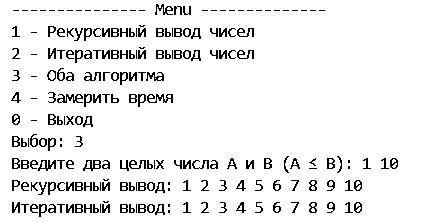
\includegraphics[width=0.8\textwidth]{images/example.png}
	\caption{Пример работы программы}
	\label{images:example}
\end{figure}

\section{Время выполнения реализаций алгоритмов}

В~таблице~\ref{tab:csv} приведены результаты замеров процессорного времени выполнения реализаций алгоритмов рекурсивного и нерекурсивного вывода чисел в диапазоне от А до В

\begin{table}[H]
	\centering
	\begin{threeparttable}
		\caption{Результаты замеров времени для рекурсивного и итеративного алгоритмов}
		\label{tab:csv}
		\begin{tabular}{|c|r|r|}
			\hline
			\textbf{Количество выводимых чисел} & \textbf{Рекурсивный, мс} & \textbf{Итеративный, мс} \\
			\hline
			100 & 0.022 & 0.019 \\
			\hline
			300 & 0.020 & 0.017 \\
			\hline
			500 & 0.024 & 0.021 \\
			\hline
			700 & 0.033 & 0.029 \\
			\hline
			900 & 0.045 & 0.038 \\
			\hline
			1100 & 0.054 & 0.047 \\
			\hline
			1300 & 0.061 & 0.054 \\
			\hline
			1500 & 0.069 & 0.060 \\
			\hline
			1700 & 0.082 & 0.071 \\
			\hline
			1900 & 0.090 & 0.078 \\
			\hline
			2100 & 0.098 & 0.084 \\
			\hline
			2300 & 0.110 & 0.096 \\
			\hline
			2500 & 0.119 & 0.104 \\
			\hline
			2700 & 0.127 & 0.112 \\
			\hline
			2900 & 0.139 & 0.119 \\
			\hline
			3100 & 0.146 & 0.127 \\
			\hline
			3300 & 0.155 & 0.135 \\
			\hline
			3500 & 0.167 & 0.143 \\
			\hline
			3700 & 0.171 & 0.150 \\
			\hline
			3900 & 0.194 & 0.171 \\
			\hline
			4100 & 0.195 & 0.171 \\
			\hline
			4300 & 0.202 & 0.178 \\
			\hline
			4500 & 0.214 & 0.187 \\
			\hline
			4700 & 0.234 & 0.206 \\
			\hline
			4900 & 0.241 & 0.208 \\
			\hline
			5100 & 0.250 & 0.218 \\
			\hline
			5300 & 0.284 & 0.247 \\
			\hline
			5500 & 0.289 & 0.251 \\
			\hline
			5700 & 0.275 & 0.240 \\
			\hline
			5900 & 0.289 & 0.250 \\
			\hline
			6000 & 0.290 & 0.253 \\
			\hline
		\end{tabular}
	\end{threeparttable}
\end{table}


По~таблице~\ref{tab:csv} был построен график представленный на~рисунке~\ref{fig:time_chart}.

\begin{figure}[H]
	\centering
	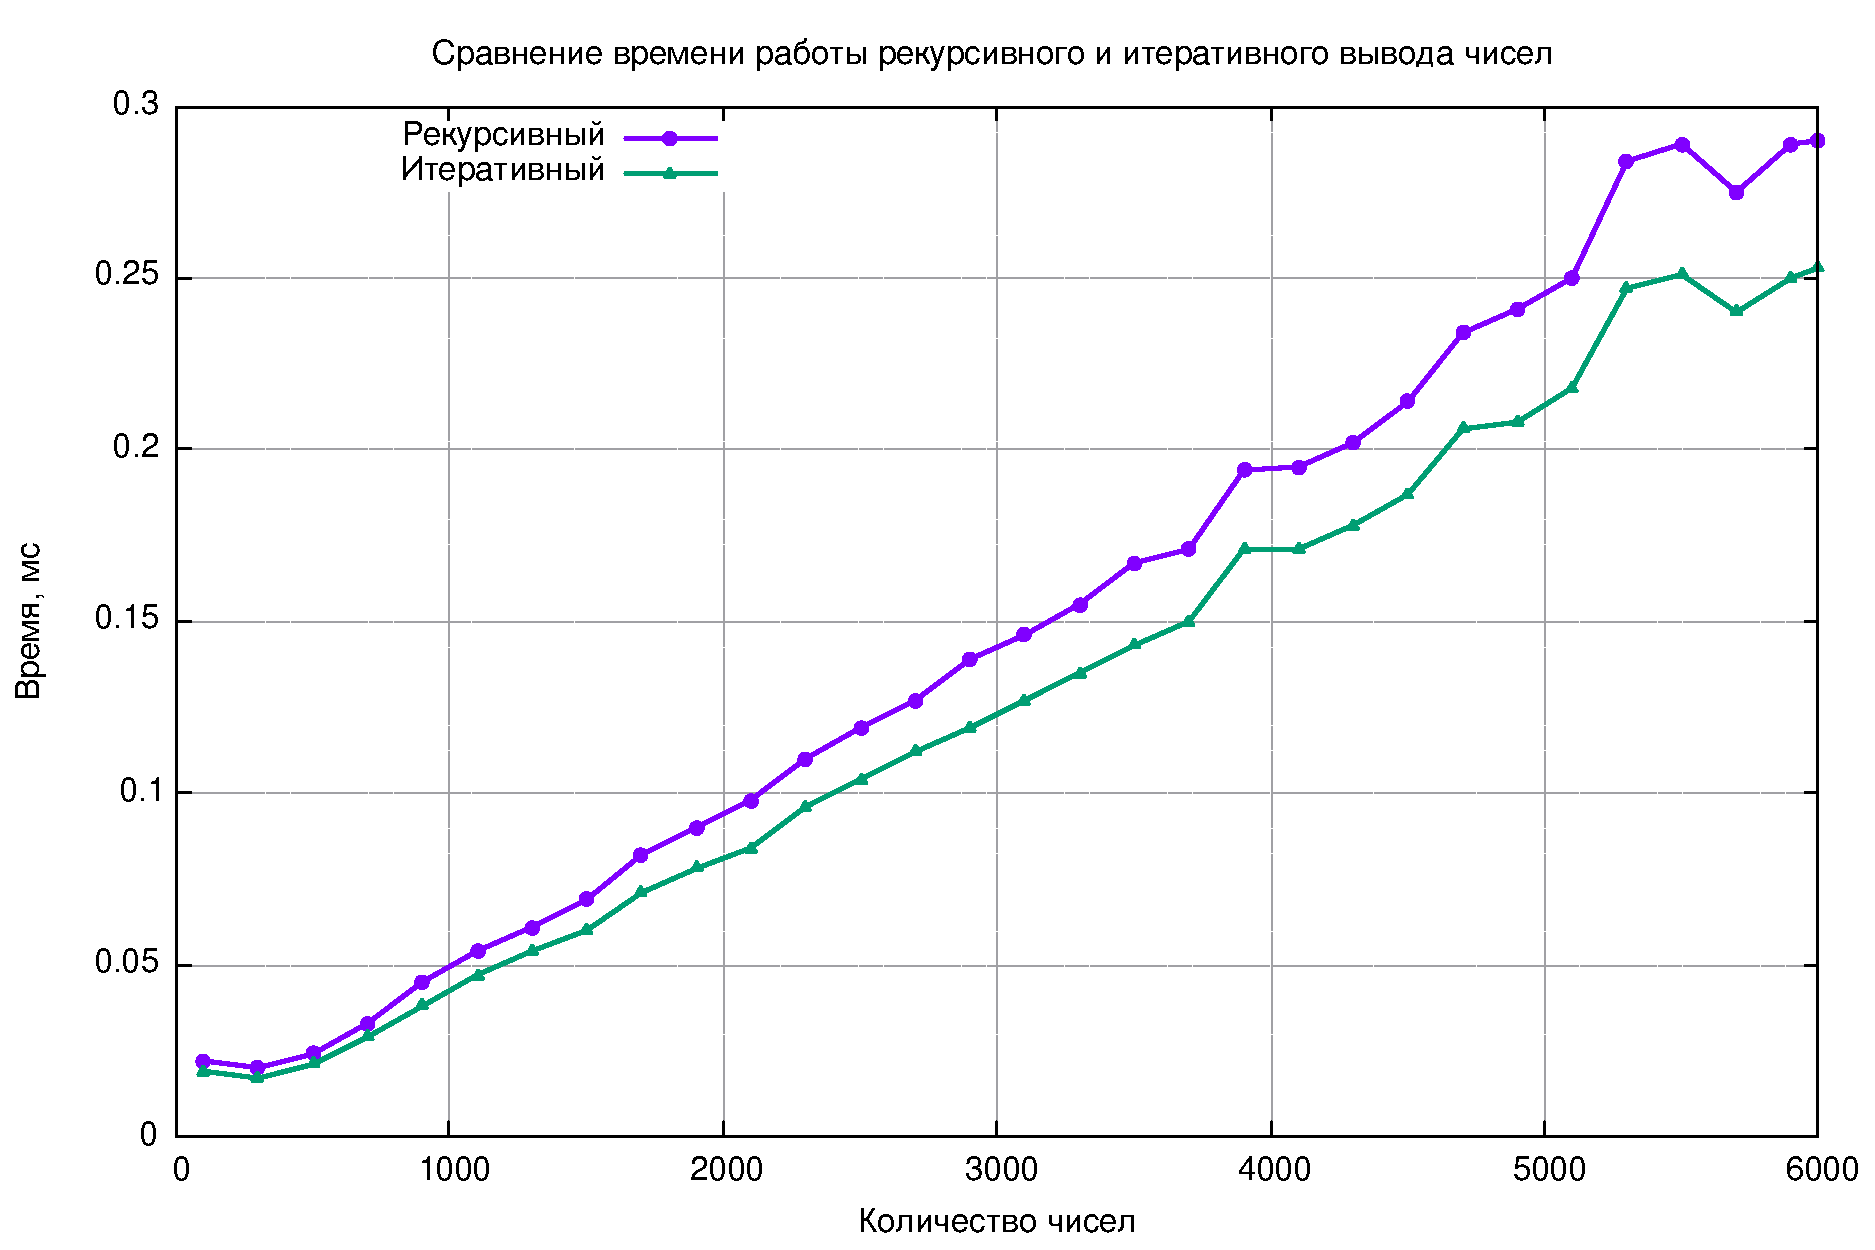
\includegraphics[width=1\textwidth]{images/test.pdf}
	\caption{График времени выполнения алгоритмов}
	\label{fig:time_chart}
\end{figure}

\section{Вывол}

Были выполнены замеры процессорного времени для рекурсивной и итеративной реализаций алгоритмов вывода чисел в диапазоне. Анализ полученных данных показал, что итеративный алгоритм демонстрирует стабильное преимущество по скорости выполнения над рекурсивным подходом.

\clearpage
